% Sostituisco i placeholder registrati con la specifica variabile per il documento corrente. Questa parte iniziale contiene intestazioni e templates.

% Modificare ad ogni modifica e documento
\newcommand{\documento}{\ST}
\newcommand{\nomedocumentofisico}{SpecificaTecnica 1\_0\_0.pdf}
\newcommand{\redazione}{\MC \\ & \DAN \\ & \AN \\ & \AS \\ & \NS}
\newcommand{\verifica}{\NS \\ & \AS}
\newcommand{\versione}{2.0.0}
\newcommand{\approvazione}{\DS}
\newcommand{\uso}{Esterno}
\newcommand{\destinateTo}{\TV, \\ & \RC, \\ & \proponente}
\newcommand{\datacreazione}{25 Febbraio 2017}
\newcommand{\datamodifica}{04 Aprile 2017}
\newcommand{\stato}{Approvato}

%Abilitazione indice delle tabelle e figure
\def\TABELLE{false}
\def\FIGURE{true}

%Inclusione di layout e variabili (Non modificare)
%Stile e dimensione del documento
\documentclass[a4paper,11pt]{article}

%Pacchetti da importare
\usepackage{ifthen}
\usepackage[italian]{babel}
\usepackage[utf8]{inputenc}
\usepackage[T1]{fontenc}
\usepackage{float}
\usepackage{chapterbib}
\usepackage{graphicx}
\usepackage[a4paper,top=2.5cm,bottom=2.5cm,left=2.5cm,right=2.5cm]{geometry}
\usepackage[colorlinks=true, urlcolor=black, citecolor=black, linkcolor=black]{hyperref}
\usepackage{booktabs}
\usepackage{fancyhdr}
\usepackage{totpages}
\usepackage{tabularx, array}
\usepackage{dcolumn}
\usepackage{epstopdf}
\usepackage{booktabs}
\usepackage{fancyhdr}
\usepackage{longtable}
\usepackage{calc}
\usepackage{datatool}
\usepackage[bottom]{footmisc}
\usepackage{listings}
\usepackage{textcomp}
\usepackage{titlesec}
\usepackage{rotating}
\usepackage{multirow}
\usepackage{placeins}
\usepackage{color}
\usepackage[table,usenames,dvipsnames]{xcolor}
\usepackage{hyperref}
\usepackage{makecell}
\usepackage{breakurl}
\usepackage{hyperref}
\usepackage{multirow}
\usepackage{xcolor,colortbl}
\usepackage{afterpage}



%Stile fancy per il documento (Header e footer)
\pagestyle{fancy}
%Rimuovo l'indentazione
\setlength{\parindent}{0pt}

%Imposto l'intestazione
\lhead{\Large{\progetto} \\ \footnotesize{\documento}}
%Linea sotto l'intestazione
\renewcommand{\headrulewidth}{0.4pt} 

%Footer
\lfoot{\textit{\gruppoLink}\\ \footnotesize{\email}}
%Footer con numero romano per le prime pagine
\rfoot{\thepage}
\cfoot{}
%Linea sopra il footer
\renewcommand{\footrulewidth}{0.4pt}   

%Imposta il livello degli elenchi 
\setcounter{secnumdepth}{7}
\setcounter{tocdepth}{7}

%Paragrafi impostati come una sezione
\titleformat{\paragraph}{\normalfont\normalsize\bfseries}{\theparagraph}{1em}{}
\titlespacing*{\paragraph}{0pt}{3.25ex plus 1ex minus .2ex}{1.5ex plus .2ex}

\titleformat{\subparagraph}{\normalfont\normalsize\bfseries}{\thesubparagraph}{1em}{}
\titlespacing*{\subparagraph}{0pt}{3.25ex plus 1ex minus .2ex}{1.5ex plus .2ex}

\makeatletter
\newcounter{subsubparagraph}[subparagraph]
\renewcommand\thesubsubparagraph{
  \thesubparagraph.\@arabic\c@subsubparagraph}
\newcommand\subsubparagraph{
  \@startsection{subsubparagraph}
    {6}
    {\parindent}
    {3.25ex \@plus 1ex \@minus .2ex}
    {0.75em}
    {\normalfont\normalsize\bfseries}}
\newcommand\l@subsubparagraph{\@dottedtocline{6}{10em}{5.5em}} 
\newcommand{\subsubparagraphmark}[1]{}
\makeatother

\makeatletter
\newcounter{subsubsubparagraph}[subsubparagraph]
\renewcommand\thesubsubsubparagraph{
  \thesubsubparagraph.\@arabic\c@subsubsubparagraph}
\newcommand\subsubsubparagraph{
  \@startsection{subsubsubparagraph}
    {7}
    {\parindent}
    {3.25ex \@plus 1ex \@minus .2ex}
    {0.75em}
    {\normalfont\normalsize\bfseries}}
\newcommand\l@subsubsubparagraph{\@dottedtocline{7}{10em}{6.5em}}
\newcommand{\subsubsubparagraphmark}[1]{}
\makeatother

%Variabili generali
\newcommand{\progetto}{API Market}
\newcommand{\gruppo}{NetBreak}
\newcommand{\gruppoLink}{\href{https://git.io/v1Rgz}{NetBreak}}
\newcommand{\email}{netbreakswe@gmail.com}

%Variabili riguardanti i documenti
\newcommand{\AdR}{Analisi dei Requisiti}
\newcommand{\NdP}{Norme di Progetto}
\newcommand{\PdP}{Piano di Progetto}
\newcommand{\SdF}{Studio di Fattibilità}
\newcommand{\PdQ}{Piano di Qualifica}
\newcommand{\VI}{Verbale Interno}
\newcommand{\VE}{Verbale Esterno}
\newcommand{\ST}{Specifica Tecnica}
\newcommand{\DDP}{Definizione di Prodotto}
\newcommand{\MU}{Manuale Utente}
\newcommand{\G}{Glossario}
\newcommand{\LdP}{Lettera di Presentazione}

%Variabili per i membri del gruppo
\newcommand{\AS}{Andrea Scalabrin}
\newcommand{\NS}{Nicolò Scapin}
\newcommand{\AN}{Alberto Nicolè}
\newcommand{\DS}{Davide Scarparo}
\newcommand{\DAN}{Dan Serbanoiu}
\newcommand{\MC}{Marco Casagrande}

%Ruoli di progetto
\newcommand{\RdP}{Responsabile di Progetto}
\newcommand{\Res}{Responsabile}
\newcommand{\Amm}{Amministratore}
\newcommand{\Ver}{Verificatore}
\newcommand{\Prog}{Progettista}
\newcommand{\Progr}{Programmatore}
\newcommand{\Ana}{Analista}
\newcommand{\RdPs}{Responsabili di Progetto}
\newcommand{\Ress}{Responsabile}
\newcommand{\Amms}{Amministratori}
\newcommand{\Vers}{Verificatori}
\newcommand{\Progs}{Progettisti}
\newcommand{\Progrs}{Programmatori}
\newcommand{\Anas}{Analisti}

%Professori e proponente
\newcommand{\TV}{Prof. Tullio Vardanega}
\newcommand{\RC}{Prof. Riccardo Cardin}
\newcommand{\IS}{ItalianaSoftware S.r.l.}
\newcommand{\proponente}{ItalianaSoftware S.r.l.}

\newcommand{\diaryEntry}[5]{#2 & \emph{#4} & #3 & #5 & #1\\ \hline}

%Comando per una nuova riga nella tabella del changelog
\newcommand{\specialcell}[2][c]{%
	\begin{tabular}[#1]{@{}c@{}}#2\end{tabular}}

\renewcommand*\sectionmark[1]{\markboth{#1}{}}
\renewcommand*\subsectionmark[1]{\markright{#1}}

%Variabili per la fase di lavoro
\newcommand{\AR}{Analisi dei Requisiti}
\newcommand{\PA}{Progettazione Architetturale}
\newcommand{\PD}{Progettazione Architetturale Dettagliata}
\newcommand{\CO}{Codifica}
\newcommand{\VV}{Verifica e Validazione}

%Variabili per le varie revisioni
\newcommand{\RR}{Revisione dei Requisiti}
\newcommand{\RP}{Revisione di Progettazione}
\newcommand{\RPMin}{Revisione di Progettazione Minima}
\newcommand{\RPMax}{Revisione di Progettazione Massima}
\newcommand{\RQ}{Revisione di Qualifica}
\newcommand{\RA}{Revisione di Accettazione}

\newcommand{\myincludegraphics}[2][]{%
	\setbox0=\hbox{\phantom{X}}%
	\vtop{
		\hbox{\phantom{X}}
		\vskip-\ht0
		\hbox{\includegraphics[#1]{#2}}}}

\renewcommand\footnoterule{\rule{\linewidth}{1pt}}

\newcommand{\nogloxy}[1]{#1} % comando da usare per evitare di metttere il mark del glossario
\newcommand{\gloxy}[1]{\emph{#1}$_G$}

\colorlet{punct}{red!60!black}
\definecolor{background}{HTML}{EEEEEE}
\definecolor{delim}{RGB}{20,105,176}
\colorlet{numb}{magenta!60!black}
\lstdefinelanguage{json}{
	basicstyle=\small\ttfamily,
	numbers=left,
	numberstyle=\scriptsize,
	stepnumber=1,
	numbersep=8pt,
	showstringspaces=false,
	breaklines=true,
	frame=lines,
	backgroundcolor=\color{background},
	literate=
	*{0}{{{\color{numb}0}}}{1}
	{1}{{{\color{numb}1}}}{1}
	{2}{{{\color{numb}2}}}{1}
	{3}{{{\color{numb}3}}}{1}
	{4}{{{\color{numb}4}}}{1}
	{5}{{{\color{numb}5}}}{1}
	{6}{{{\color{numb}6}}}{1}
	{7}{{{\color{numb}7}}}{1}
	{8}{{{\color{numb}8}}}{1}
	{9}{{{\color{numb}9}}}{1}
	{:}{{{\color{punct}{:}}}}{1}
	{,}{{{\color{punct}{,}}}}{1}
	{\{}{{{\color{delim}{\{}}}}{1}
	{\}}{{{\color{delim}{\}}}}}{1}
	{[}{{{\color{delim}{[}}}}{1}
	{]}{{{\color{delim}{]}}}}{1},
}
\lstset{language=json}
\lstset{literate=%
	{Ö}{{\"O}}1
	{Ä}{{\"A}}1
	{Ü}{{\"U}}1
	{é}{{\"s}}1
	{è}{{\"e}}1
	{à}{{\"a}}1
	{ö}{{\"o}}1
}

\newcommand{\impl}{\textcolor{Green}{Implementato}}
\newcommand{\implno}{\textcolor{Red}{Non Implementato}}
\newcommand\Tstrut{\rule{0pt}{3.2ex}}         % = `top' strut
\newcommand\Bstrut{\rule[-1.9ex]{0pt}{0pt}}   % = `bottom' strut
\definecolor{Gray}{gray}{0.85}
\usepackage[inline]{enumitem}

%Inclusione del changelog per il documento corrente
\newcommand{\modifiche}
{	
	Approvazione documento & \specialcell[t]{\DS\\\Res} & \specialcell[t]{2017-03-04\\2.0.0}
	\\
	\hline
	Verifica documento & \specialcell[t]{\MC\\\Ver} & \specialcell[t]{2017-03-03\\1.1.0}
	\\
	\hline
	Stesura sezione "Resoconto attività di verifica" & \specialcell[t]{\DS\\\Ana} & \specialcell[t]{2017-03-01\\1.0.4}
	\\
	\hline
	Nuova stesura sezione "Qualità di prodotto" & \specialcell[t]{\NS\\\Ana} & \specialcell[t]{2017-02-28\\1.0.3}
	\\
	\hline
	Nuova stesura sezione "Qualità di processo" & \specialcell[t]{\DS\\\Ana} & \specialcell[t]{2017-02-24\\1.0.2}
	\\
	\hline
	Ristrutturazione documento secondo suggerimenti del committente & \specialcell[t]{\DS\\\Ana} & \specialcell[t]{2017-02-23\\1.0.1}
	\\
	\hline
	Approvazione documento & \specialcell[t]{\NS\\\Res} & \specialcell[t]{2017-01-03\\1.0.0}
	\\
	\hline
	Effettuate modifiche secondo verifica & \specialcell[t]{\DS\\\Ana} & \specialcell[t]{2016-12-31\\0.1.1}
	\\
	\hline
	Verifica documento & \specialcell[t]{\MC\\\Ver} & \specialcell[t]{2016-12-29\\0.1.0}
	\\
	\hline
	Creata sezione "Qualità di prodotto" & \specialcell[t]{\DS\\\Ana} & \specialcell[t]{2016-12-28\\0.0.5}
	\\
	\hline
	Creata sezione "Qualità di processo" & \specialcell[t]{\DAN\\\Ana} & \specialcell[t]{2016-12-26\\0.0.4}
	\\
	\hline
	Creata sezione "Definizione obiettivi di qualità" & \specialcell[t]{\AN\\\Ana} & \specialcell[t]{2016-12-23\\0.0.3}
	\\
	\hline
	Creata introduzione & \specialcell[t]{\AN\\\Ana} & \specialcell[t]{2016-12-22\\0.0.2}
	\\
	\hline	
	Creato template documento & \specialcell[t]{\AS\\\Res} & \specialcell[t]{2016-12-20\\0.0.1}
	\\	
	
}


%Imposto la profondità degli indici
\setcounter{secnumdepth}{8}
\setcounter{tocdepth}{8}





\begin{document}

%Inclusione del template per la homepage (Non modificare)
%Importante: Non modificare questo template
%Modificare il documento principale per cambiare le parti

\begin{center}


%Spaziatura verticale

\vspace{4em}

%Intestazione con nome del gruppo
\begin{center} 
	\begin{Huge}
		\textbf{\fontsize{15mm}{20mm}\selectfont \gruppoLink} 
	\end{Huge}
\end{center}

\begin{center}
	\begin{Large}
		\vspace{0.3em}
		\textbf{Progetto \progetto}
	\end{Large}
\end{center}

%Inclusione del logo

\includegraphics[keepaspectratio = true,width=6cm]{../../Template/img/LogoNetbreak.png}

%Prima pagina senza intestazione né piè di pagina	
\thispagestyle{empty}

%Le informazioni del documento sono ancorate a fine pagina
\vfill

%Nome del documento
\begin{Huge} \textbf{\documento} \end{Huge}

%Tabella centrale
\begin{center}
\large\textbf{Informazioni sul documento} \\ \vspace{2em}
\small
\begin{tabular}{r l}
	\textbf{Nome del file} & \nomedocumentofisico \\
	\textbf{Data di creazione} & \datacreazione\\
	\textbf{Ultima modifica e versione} & \datamodifica\\ & Versione \versione\\
	\textbf{Stato} & \stato \\
	\textbf{Redatto da}	& \redazione\\
	\textbf{Verificato da}	& \verifica\\
	\textbf{Approvato da}	& \approvazione\\
	\textbf{Uso}  & \uso\\
	\textbf{Distribuzione} & \gruppo \\
	\textbf{Destinato a}  &  \destinateTo \\
\end{tabular}
\end{center}

\vspace{2em}

\normalsize
%Inclusione abstract
\textbf{Abstract\\} 


\end{center}
\clearpage


%Registro delle modifiche e indice (Non modificare)
\pagenumbering{Roman}
\newpage
%Tabulazione per il changelog multipagina
%Utilizzare la variabile relativa alla pagina corrispondente
%Per indicare la tabella corrispondente

\begin{center}
	\Large{\textbf{Changelog}}
	\\\vspace{0.5cm}
	\normalsize
	\begin{tabularx}{\textwidth}{Xcc}
		\textbf{Descrizione} & \textbf{Autore e Ruolo} & \textbf{Data e versione} \\\toprule
		\modificheuno
		\bottomrule
	\end{tabularx}
	\newpage
	\begin{tabularx}{\textwidth}{Xcc}
		\textbf{Descrizione} & \textbf{Autore e Ruolo} & \textbf{Data e versione} \\\toprule
		\modifichedue
		\bottomrule
	\end{tabularx}
\end{center}
\newpage
\newpage
%Inserisce il link all'indice
%\addcontentsline{toc}{section}{Indice}
\newpage
\tableofcontents
\clearpage 

%Se è stata impostata a true la variabile per la lista delle tabelle, la mostra
\ifthenelse{\equal{\TABELLE}{true}} 
{\listoftables \newpage}{}

%Se è stata impostata a true la variabile per la lista delle figure, la mostra
\ifthenelse{\equal{\FIGURE}{true}}
{\listoffigures \newpage}{}

%Da qui comincia la numerazione normale
\pagenumbering{arabic}

%Imposta il formato di visualizzazione
\rfoot{\thepage~di~\pageref{TotPages}}

%Inclusione delle varie sezioni di contenuto
%Introduzione e contenuti di ogni tipo

\newpage
\section{Introduzione}

\subsection{Scopo del documento}
Questo documento descrive le scelte e le strategie attuate per permettere di raggiungere determinati obiettivi di qualità misurabili. A questo scopo, sarà necessario un continuo processo di Verifica, orientato ad individuare e correggere errori ed eventuali sprechi di risorse.
Per conseguire dei risultati concreti, il processo di Verifica dovrà fornire dei dati quantificabili per poter valutare se gli obiettivi sono stati raggiunti o meno. Per facilitarne la valutazione, per ogni metrica sarannno indicati due range:
\begin{itemize}
	\item \textbf{Range accettazione:} rappresenta l'intervallo di valori minimi richiesti per il raggiungimento degli obiettivi di qualità definiti;
	\item \textbf{Range ottimale:} rappresenta l'intervallo di valori desiderati, entro cui dovrebbe collocarsi la misurazione. Nel caso in cui non si rientrasse in questo range, sarà necessario effettuare una verifica più accurata, al fine di individuarne le cause e poter applicare le dovute correzioni.
\end{itemize}

\subsection{Scopo del prodotto}
Lo scopo del prodotto è la realizzazione di un \textit{API Market\ped{G}} per l'acquisto e la vendita di \textit{microservizi\ped{G}}. Il sistema offrirà la possibilità di registrare nuove \textit{API\ped{G}} per la vendita, permetterà la consultazione e la ricerca di API ai potenziali acquirenti, gestendo i permessi di accesso ed utilizzo tramite creazione e controllo di relative \textit{API key\ped{G}}. Il sistema, oltre alla web app stessa, sarà corredato di un \textit{API Gateway\ped{G}} per la gestione delle richieste e il controllo delle chiavi, e fornirà funzionalità avanzate di statistiche per il gestore della piattaforma e per i fornitori dei microservizi.

\subsection{Riferimenti normativi}
\begin{itemize}
\item \textsc{NormeDiProgetto 3\_0\_0.pdf};
\item \textbf{Capitolato d’appalto C1:} APIM: An API Market Platform\\ \url{http://www.math.unipd.it/~tullio/IS-1/2016/Progetto/C1.pdf};
\end{itemize}

\subsection{Riferimenti informativi}
\begin{itemize}
	\item \textsc{PianoDiProgetto 3\_0\_0.pdf};
	\item \textbf{Slide del corso riguardo la qualità di prodotto}\\ \url{http://www.math.unipd.it/~tullio/IS-1/2016/Dispense/L10.pdf};
	\item \textbf{Slide del corso riguardo la qualità di processo}\\ \url{http://www.math.unipd.it/~tullio/IS-1/2016/Dispense/L11.pdf};
	\item \textbf{Standard ISO/IEC 12207:2008}\\ \url{https://www.iso.org/obp/ui/#iso:std:iso-iec:12207:ed-2:v1:en};
	\item \textbf{Standard ISO 9001}\\ \url{https://www.iso.org/iso-9001-quality-management.html};
	\item \textbf{Standard ISO/IEC 9126:2001}\\ \url{https://en.wikipedia.org/wiki/ISO/IEC_9126};
	\item \textbf{Standard ISO/IEC 15504}\\ \url{https://en.wikipedia.org/wiki/ISO/IEC_15504};
	\item \textbf{Indice Gulpease}\\ \url{https://it.wikipedia.org/wiki/Indice_Gulpease};	
\end{itemize}

\subsection{Glossario}
Per semplificare la consultazione e disambiguare alcune terminologie tecniche, le voci indicate con la lettera \textit{G} a pedice sono descritte approfonditamente nel documento \textsc{Glossario 3\_0\_0.pdf} e specificate solo alla prima occorrenza all'interno del suddetto documento.
\newpage
\section{Specifica del prodotto}

\subsection{Architettura generale}

\subsection{Pattern architetturale}


\newpage
\section{Tecnologie utilizzate}
In questa sezione, vengono descritte le tecnologie utilizzate per la realizzazione della piattaforma. Verranno elencati i pregi e i difetti individuati durante l'analisi, e le motivazioni che hanno spinto il \textit{gruppo NetBreak} a intraprendere tali scelte progettuali e tecnologiche.

\subsection{Angular 2}

\subsection{Bootstrap 3}

\subsection{CSS3}

\subsection{HTML5}

\subsection{Java}

\subsection{Javascript ES6}

\subsection{Jolie}

\subsection{JQuery}

\subsection{Leonardo}

\subsection{Meteor}

\subsection{PostgreSQL}




\newpage
\section{Design pattern utilizzati}

\subsection{Aggregator}




\newpage
\section{Diagrammi dei packages e delle classi}

\subsection{Introduzione}
Questa sezione racchiude i diagrammi dei packages, raccolti tramite un approccio top-down. \textbf{N.B.: raggiunto il sub-package minimo, si procederà con la descrizione delle classi implementate al suo interno}.\\Considerando l'approccio adottato e il particolare applicativo realizzato con un pattern a microservizi, il team non si discosterà dalla nomenclatura tradizionale di \textit{Classe}, intesa come una categoria di entità in grado di svolgere uno specifico compito. Per mantenere una conformità con lo standard UML, dunque, verrà utilizzato il termine \textit{classe} per indicare ciò che all'atto pratico sarà implementato come un microservizio vero e proprio, stand-alone, con i propri metodi, in grado di fornire la funzionalità preposta. Trattandosi di una progettazione con un livello di dettaglio intermedio, le classi non verranno definite, bensì verrà data una descrizione della loro funzionalità, lo scopo e le relazioni che intercorrono con le altre classi. Tale descrizione sarà integrata nella seguente descrizione dei packages al livello più basso dell'elenco.

L'applicativo API Market è strutturato, come di consueto, in un lato front-end ed un lato back-end, come mostrato dal diagramma seguente:

\begin{figure}[H]
	\centering
	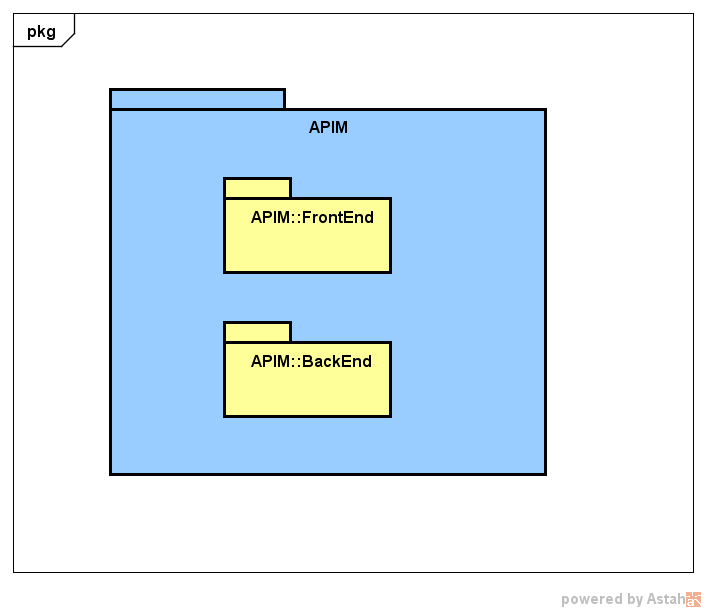
\includegraphics
	[width=0.7\linewidth]
	{UML/DiagrammiPackage/APIM.png}
	\caption{Package APIM}
\end{figure}

\newpage
\subsection{Front-end}

Il lato front-end risulta così strutturato:

\begin{figure}[H]
	\centering
	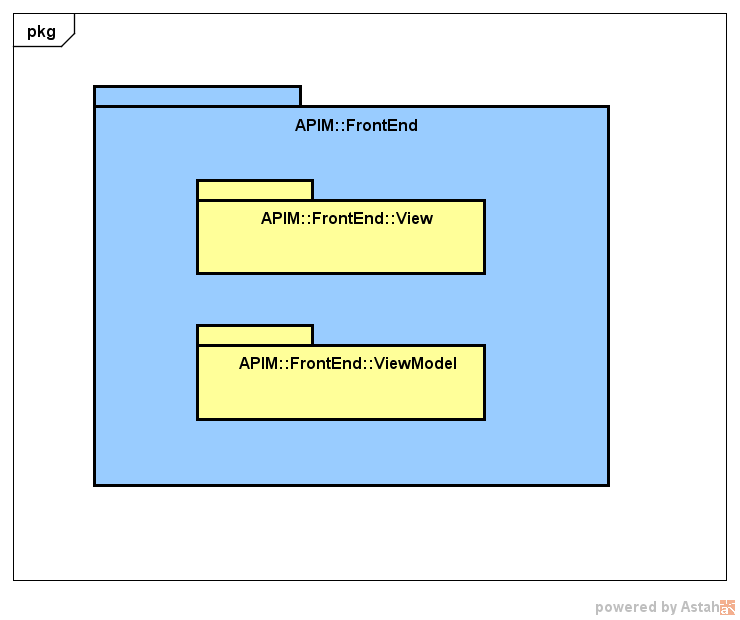
\includegraphics
	[width=0.7\linewidth]
	{UML/DiagrammiPackage/FrontEnd.png}
	\caption{Package APIM::FrontEnd}
\end{figure}

Nella parte front-end sono, dunque, presenti i package View e ViewModel, che rispecchiano l'architettura nativa dei framework scelti.

\begin{minipage}{\linewidth}
\subsubsection{View}

Il package per la componente View contiene i seguenti sub-packages:

\begin{figure}[H]
	\centering
	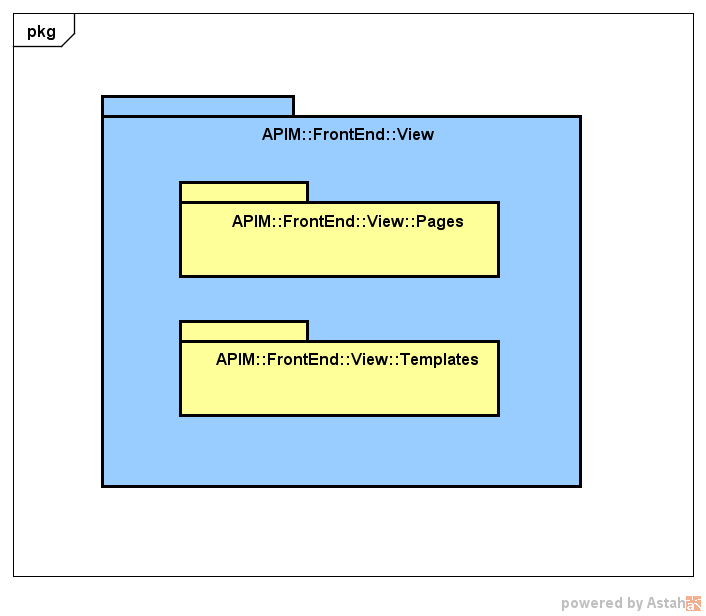
\includegraphics
	[width=0.7\linewidth]
	{UML/DiagrammiPackage/View.png}
	\caption{Package APIM::FrontEnd::View}
\end{figure}

\begin{itemize}
	\item \textbf{Pages}: il package \textit{Pages} contiene una classe astratta \textit{Page}. Essa è utilizzabile tramite una derivazione concreta di tale classe, e l'implementazione avviene a seconda di ciò che è necessario visualizzare. Tali implementazioni possono usufruire dei template, per gestire situazioni standardizzate.
	\item \textbf{Templates}: il package \textit{Templates} contiene un modello standard delle componenti utilizzabili per la rappresentazione. Ogni pagina che presenta situazioni e modelli analoghi può utilizzare un template già definito, per un maggior riuso, e per distinguere nettamente gli elementi contenuti in una pagina dalla loro realizzazione.
\end{itemize}
\end{minipage}

\paragraph{Pages}

\begin{figure}[H]
	\centering
	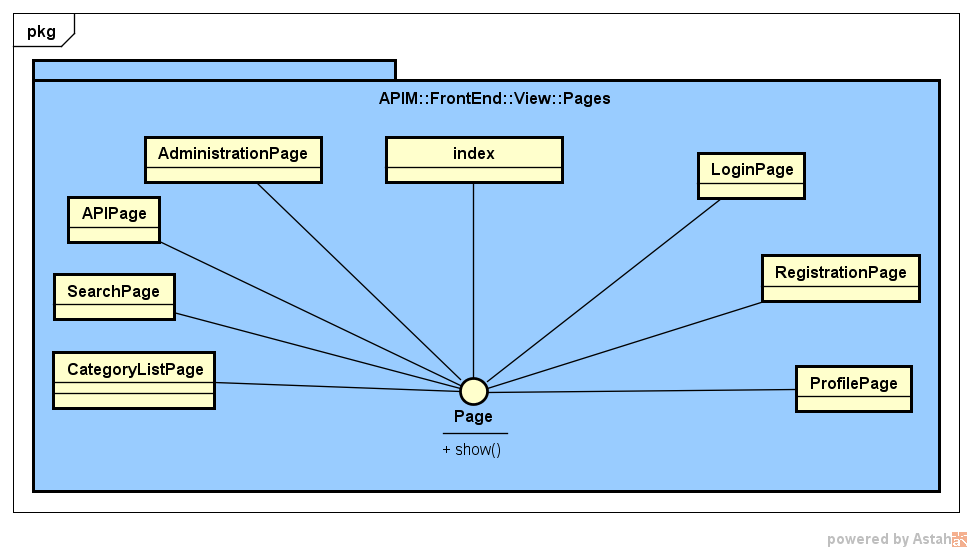
\includegraphics
	[width=0.7\linewidth]
	{UML/DiagrammiPackage/Pages.png}
	\caption{Package APIM::FrontEnd::View::Pages}
\end{figure}

\subparagraph{Page}
\begin{itemize}
	\item \textbf{Funzione del componente}: rappresenta una pagina web;
	\item \textbf{Relazioni d’uso di altri componenti}: interfaccia di base da cui derivano le altre pagine web;
	\item \textbf{Attività svolte e dati trattati}: definisce le caratteristiche minime che ogni pagina deve possedere.
\end{itemize}

\subparagraph{Index}
\begin{itemize}
	\item \textbf{Funzione del componente}: rappresenta la pagina principale dell'API Market;
	\item \textbf{Relazioni d’uso di altri componenti}: concretizza l'interfaccia \textit{Page} e utilizza i template \textit{MainMenu} e \textit{SearchForm};
	\item \textbf{Attività svolte e dati trattati}: permette l'autenticazione dell'utente e permette a un utente non autenticato di consultare una lista di API.
\end{itemize}

\subparagraph{LoginPage}
\begin{itemize}
	\item \textbf{Funzione del componente}: rappresenta la pagina di login;
	\item \textbf{Relazioni d’uso di altri componenti}: concretizza l'interfaccia \textit{Page} e utilizza i template \textit{MainMenu}, \textit{LoginForm}, \textit{PasswordRecoveryForm};
	\item \textbf{Attività svolte e dati trattati}: permette l'autenticazione dell'utente o il recupero della sua password.
\end{itemize}

\subparagraph{RegistrationPage}
\begin{itemize}
	\item \textbf{Funzione del componente}: rappresenta la pagina di registrazione;
	\item \textbf{Relazioni d’uso di altri componenti}: concretizza l'interfaccia \textit{Page} e utilizza il template \textit{MainMenu}, \textit{RegistrationForm};
	\item \textbf{Attività svolte e dati trattati}: permette la registrazione di un utente.
\end{itemize}

\subparagraph{ProfilePage}
\begin{itemize}
	\item \textbf{Funzione del componente}: rappresenta la pagina dove sono presenti le informazioni del profilo di un utente;
	\item \textbf{Relazioni d’uso di altri componenti}: concretizza l'interfaccia \textit{Page} e utilizza i template \textit{MainMenu}, \textit{ProfileForm}, \textit{EditProfileForm}, \textit{UserMenu}, \textit{TransactionList}, \textit{Transaction}, \textit{MyAPIList};
	\item \textbf{Attività svolte e dati trattati}: permette la consultazione dei dati di profilo a un utente registrato, la modifica dei dati del profilo, la visualizzazione delle API acquistate o registrate come lista o in dettaglio.
\end{itemize}

\subparagraph{AdministrationPage}
\begin{itemize}
	\item \textbf{Funzione del componente}: rappresenta la pagina di un amministratore;
	\item \textbf{Relazioni d’uso di altri componenti}: concretizza l'interfaccia \textit{Page} e utilizza il template \textit{MainMenu}, \textit{TransactionList}, \textit{UserList}, \textit{User}, \textit{TransactionList}, \textit{Transaction}, \textit{SearchForm}, \textit{SearchResult};
	\item \textbf{Attività svolte e dati trattati}: permette ad un amministratore di moderare gli utenti, vedere una lista di utenti e di API con possibilità di rimuovere un utente o un'API, ed effettuare una ricerca su utenti o API, vedendone il risultato.
\end{itemize}

\subparagraph{APIPage}
\begin{itemize}
	\item \textbf{Funzione del componente}: rappresenta la pagina di un'API o di una lista di API;
	\item \textbf{Relazioni d’uso di altri componenti}: concretizza l'interfaccia \textit{Page} e utilizza i template \textit{MainMenu}, \textit{APIList}, \textit{API}, \textit{SearchResult}, \textit{MyAPIList}, \textit{APIRegistrationForm}, \textit{APIEditForm}, \textit{CheckoutForm}, \textit{SearchForm}, \textit{SearchResult};
	\item \textbf{Attività svolte e dati trattati}: permette a un utente di consultare i dati di un'API, di ricercare un'API e vederne il risultato a schermo, consultare un lista di proprie API acquistate o registrate, e se le API sono proprie registrate, consente di modificarle. \MakeUppercase{è} possibile acquistare un'API e portare a termine l'acquisto tramite un form apposito.
\end{itemize}

\subparagraph{SearchPage}
\begin{itemize}
	\item \textbf{Funzione del componente}: rappresenta la pagina di ricerca;
	\item \textbf{Relazioni d’uso di altri componenti}: concretizza l'interfaccia \textit{Page} e utilizza i template \textit{MainMenu}, \textit{SearchForm} e \textit{SearchResult};
	\item \textbf{Attività svolte e dati trattati}: permette la ricerca di un'API o di un utente.	
\end{itemize}

\subparagraph{CategoryListPage}
\begin{itemize}
	\item \textbf{Funzione del componente}: rappresenta la pagina di una categoria;
	\item \textbf{Relazioni d’uso di altri componenti}: concretizza l'interfaccia \textit{Page} e utilizza i template \textit{MainMenu}, \textit{CategoryList} e \textit{Category};
	\item \textbf{Attività svolte e dati trattati}: permette la consultazione di un'API per categoria.
\end{itemize}


\paragraph{Templates}

\begin{figure}[H]
	\centering
	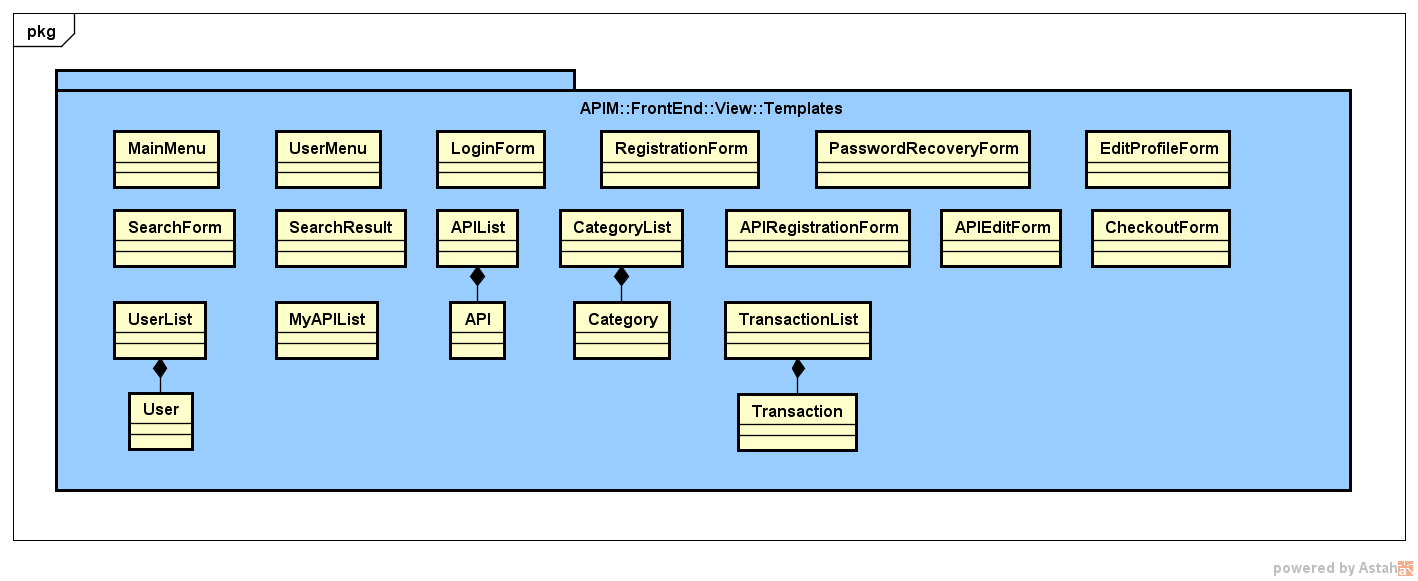
\includegraphics
	[width=0.7\linewidth]
	{UML/DiagrammiPackage/Templates.png}
	\caption{Package APIM::FrontEnd::View::Templates}
\end{figure}

\subparagraph{MainMenu}
\begin{itemize}
	\item \textbf{Funzione del componente}: rappresenta il template del menu principale;
	\item \textbf{Relazioni d’uso di altri componenti}: tutte le pagine derivate da \textit{Page};
	\item \textbf{Attività svolte e dati trattati}: è lo scheletro del menu che sarà presente su ogni pagina. Una sua modifica si rifletterà su tutte le view.
\end{itemize}

\subparagraph{UserMenu}
\begin{itemize}
	\item \textbf{Funzione del componente}: rappresenta il template del menu utente;
	\item \textbf{Relazioni d’uso di altri componenti}: tutte le pagine derivate da \textit{Page} di un utente autenticato;
	\item \textbf{Attività svolte e dati trattati}: è lo scheletro del menu utente.
\end{itemize}

\subparagraph{LoginForm}
\begin{itemize}
	\item \textbf{Funzione del componente}: rappresenta il template del form per il login;
	\item \textbf{Relazioni d’uso di altri componenti}: \textit{LoginPage};
	\item \textbf{Attività svolte e dati trattati}: è lo scheletro del form che sarà usato per autenticarsi all'applicazione web.
\end{itemize}

\subparagraph{RegistrationForm}
\begin{itemize}
	\item \textbf{Funzione del componente}: rappresenta il template del form per la registrazione;
	\item \textbf{Relazioni d’uso di altri componenti}: \textit{RegistrationPage};
	\item \textbf{Attività svolte e dati trattati}: è lo scheletro del form che sarà usato per registrarsi all'applicazione web.
\end{itemize}

\subparagraph{PasswordRecoveryForm}
\begin{itemize}
	\item \textbf{Funzione del componente}: rappresenta il template del form per il recupero della password;
	\item \textbf{Relazioni d’uso di altri componenti}: \textit{LoginPage};
	\item \textbf{Attività svolte e dati trattati}: è lo scheletro del form che sarà usato per recuperare la password.
\end{itemize}

\subparagraph{EditProfileForm}
\begin{itemize}
	\item \textbf{Funzione del componente}: rappresenta il template del form per la modifica del profilo utente;
	\item \textbf{Relazioni d’uso di altri componenti}: \textit{ProfilePage};
	\item \textbf{Attività svolte e dati trattati}: è lo scheletro del form che sarà usato per modificare il profilo.
\end{itemize}

\subparagraph{SearchForm}
\begin{itemize}
	\item \textbf{Funzione del componente}: rappresenta il template del form per la ricerca;
	\item \textbf{Relazioni d’uso di altri componenti}: \textit{SearchPage};
	\item \textbf{Attività svolte e dati trattati}: è lo scheletro del form che sarà usato per la ricerca.
\end{itemize}

\subparagraph{SearchResultForm}
\begin{itemize}
	\item \textbf{Funzione del componente}: rappresenta il template del form per visualizzare i risultati della ricerca;
	\item \textbf{Relazioni d’uso di altri componenti}: \textit{SearchPage};
	\item \textbf{Attività svolte e dati trattati}: è lo scheletro del form che sarà usato per visualizzare i risultati della ricerca.
\end{itemize}

\subparagraph{API}
\begin{itemize}
	\item \textbf{Funzione del componente}:  rappresenta il template della view usata per visualizzare i dati di un'API;
	\item \textbf{Relazioni d’uso di altri componenti}: \textit{APIPage};
	\item \textbf{Attività svolte e dati trattati}: è lo scheletro della view che sarà usata per visualizzare i dati di un'API.
\end{itemize}

\subparagraph{APIList}
\begin{itemize}
	\item \textbf{Funzione del componente}: rappresenta il template della view usata per visualizzare una lista di API;
	\item \textbf{Relazioni d’uso di altri componenti}: \textit{APIPage};
	\item \textbf{Attività svolte e dati trattati}: è lo scheletro della view che sarà usata per visualizzare una lista di API.
\end{itemize}

\subparagraph{Category}
\begin{itemize}
	\item \textbf{Funzione del componente}: rappresenta il template di una categoria;
	\item \textbf{Relazioni d’uso di altri componenti}: \textit{CategoryListPage};
	\item \textbf{Attività svolte e dati trattati}: \`{e} lo scheletro della view che sar\`{a} usata per visualizzare una categoria.
\end{itemize}

\subparagraph{CategoryList}
\begin{itemize}
	\item \textbf{Funzione del componente}: rappresenta il template della view che sar\`{a} usata per visualizzare una lista di categorie;
	\item \textbf{Relazioni d’uso di altri componenti}: \textit{CategoryListPage};
	\item \textbf{Attività svolte e dati trattati}: \`{e} lo scheletro della view che sar\`{a} usata per visualizzare una lista di categorie.
\end{itemize}

\subparagraph{APIRegistrationForm}
\begin{itemize}
	\item \textbf{Funzione del componente}: rappresenta il template del form per la registrazione di un'API;
	\item \textbf{Relazioni d’uso di altri componenti}: \textit{RegistrationPage};
	\item \textbf{Attività svolte e dati trattati}: \`{e} lo scheletro del form che sar\`{a} usato per la registrazione di un'API.
\end{itemize}

\subparagraph{APIEditForm}
\begin{itemize}
	\item \textbf{Funzione del componente}: rappresenta il template del form per modificare un'API;
	\item \textbf{Relazioni d’uso di altri componenti}: \textit{APIPage};
	\item \textbf{Attività svolte e dati trattati}: \`{e} lo scheletro del form che sar\`{a} usato per la modifica di un'API.
\end{itemize}

\subparagraph{CheckoutForm}
\begin{itemize}
	\item \textbf{Funzione del componente}: rappresenta il template del form per effettuare il checkout per l'acquisto un'API;
	\item \textbf{Relazioni d’uso di altri componenti}: \textit{APIPage};
	\item \textbf{Attività svolte e dati trattati}: \`{e} lo scheletro del form che sar\`{a} usato per effettuare il checkout per l'acquisto un'API.
\end{itemize}

\subparagraph{User}
\begin{itemize}
	\item \textbf{Funzione del componente}: rappresenta il template di un utente;
	\item \textbf{Relazioni d’uso di altri componenti}: \textit{AdministrationPage};
	\item \textbf{Attività svolte e dati trattati}: \`{e} lo scheletro della view che sar\`{a} usata per visualizzare un utente o i suoi dati.
\end{itemize}

\subparagraph{UserList}
\begin{itemize}
	\item \textbf{Funzione del componente}: rappresenta il template di una lista di utenti;
	\item \textbf{Relazioni d’uso di altri componenti}: \textit{AdministrationPage};
	\item \textbf{Attività svolte e dati trattati}: \`{e} lo scheletro della view che sar\`{a} usata per visualizzare una lista di utenti e i dati a loro pertinenti.
\end{itemize}

\subparagraph{MyAPIList}
\begin{itemize}
	\item \textbf{Funzione del componente}: rappresenta il template di una lista di API;
	\item \textbf{Relazioni d’uso di altri componenti}: \textit{APIPage}, \textit{ProfilePage};
	\item \textbf{Attività svolte e dati trattati}: \`{e} lo scheletro della view che sar\`{a} usata per visualizzare una lista di API e i dati a loro pertinenti.
\end{itemize}

\subparagraph{Transaction}
\begin{itemize}
	\item \textbf{Funzione del componente}: rappresenta il template di una transazione;
	\item \textbf{Relazioni d’uso di altri componenti}: \textit{ProfilePage}, \textit{AdministrationPage};
	\item \textbf{Attività svolte e dati trattati}: \`{e} lo scheletro della view che sar\`{a} usata per visualizzare una transazione e i dati a essa pertinenti.
\end{itemize}

\subparagraph{TransactionList}
\begin{itemize}
	\item \textbf{Funzione del componente}: rappresenta il template di una lista di transazioni;
	\item \textbf{Relazioni d’uso di altri componenti}: \textit{ProfilePage}, \textit{AdministrationPage};
	\item \textbf{Attività svolte e dati trattati}: \`{e} lo scheletro della view che sar\`{a} usata per visualizzare una lista di transazioni e i dati a loro pertinenti.
\end{itemize}

\begin{minipage}{\linewidth}
\subsubsection{ViewModel}

Il package per la componente ViewModel contiene i seguenti sub-packages:

\begin{figure}[H]
	\centering
	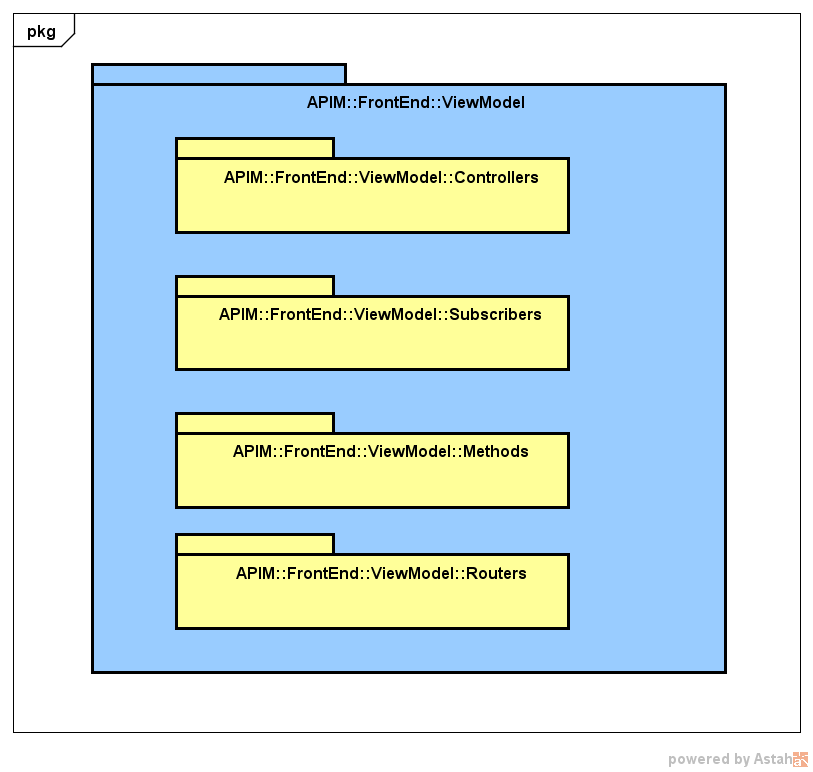
\includegraphics
	[width=0.7\linewidth]
	{UML/DiagrammiPackage/ViewModel.png}
	\caption{Package APIM::FrontEnd::ViewModel}
\end{figure}

La componente \textit{ViewModel} ha il compito di realizzare il data-binding con i componenti della \textit{View}, interagendo con la componente \textit{Model}, la quale fornisce i dati e ne permette la modifica. La componente \textit{Model} è parte del lato back-end della piattaforma, sebbene adottando un tale approccio si ha una linea di demarcazione meno netta tra le due parti. Di seguito, si analizzano i packages contenuti all'interno del componente \textit{ViewModel}:

\begin{itemize}
	\item \textbf{Controllers}: contiene i controller necessari alle views per comunicare con il \textit{Model};
	\item \textbf{Subscribers}: contiene le classi necessarie al subscribing alle collezioni pubblicate dai \textit{Publisher};
	\item \textbf{Methods}: contiene le classi necessarie a MeteorJS per la corretta fruizione dei dati;
	\item \textbf{Routers}: contiene la classe che esegue il routing dell'intera applicazione. 
\end{itemize}
\end{minipage}

\paragraph{Controllers}

\begin{figure}[H]
	\centering
	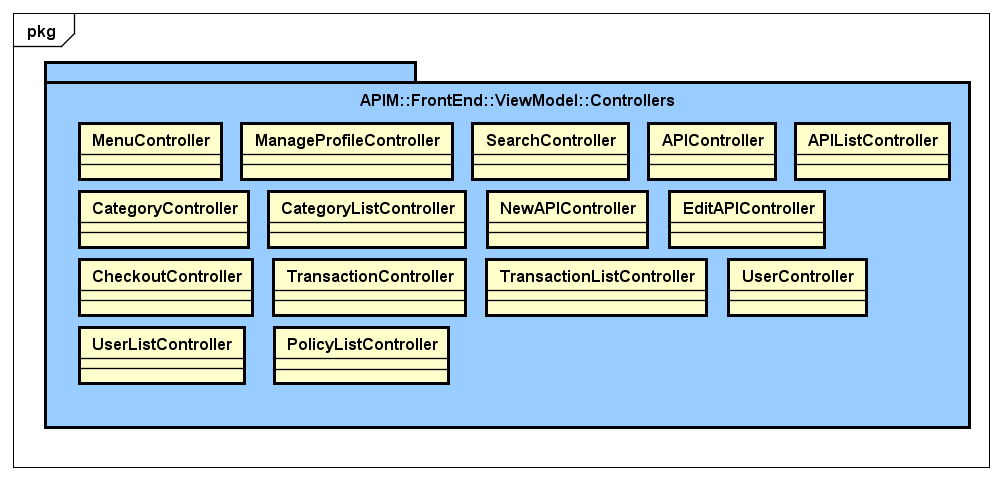
\includegraphics
	[width=0.7\linewidth]
	{UML/DiagrammiPackage/Controllers.png}
	\caption{Package APIM::FrontEnd::ViewModel::Controllers}
\end{figure}

\subparagraph{MenuController}
\begin{itemize}
	\item \textbf{Funzione del componente}: la classe permette la corretta visualizzazione del menu, in base ai propri privilegi;
	\item \textbf{Relazioni d’uso di altri componenti}: il controller è collegato ai template \textit{MainMenu} e \textit{UserMenu}.
\end{itemize}

\subparagraph{ManageProfileController}
\begin{itemize}
	\item \textbf{Funzione del componente}: permette la gestione del proprio profilo utente;
	\item \textbf{Relazioni d’uso di altri componenti}: utilizza i template \textit{TransactionList}, \textit{Transaction}, \textit{EditProfileForm}, \textit{MyAPIList};
	\item \textbf{Attività svolte e dati trattati}: coordina tutte le funzionalità di gestione che può svolgere un utente registrato, come gestire le proprie transazioni e vedere lo stato dei suoi abbonamenti. 
\end{itemize}

\subparagraph{SearchController}
\begin{itemize}
	\item \textbf{Funzione del componente}: permette la gestione della ricerca;
	\item \textbf{Relazioni d’uso di altri componenti}: utilizza i template \textit{SearchForm}, \textit{SearchResult};
	\item \textbf{Attività svolte e dati trattati}: coordina tutte le funzionalità di ricerca che può svolgere un utente non registrato o registrato, in base ai privilegi annessi.
\end{itemize}

\subparagraph{APIController}
\begin{itemize}
	\item \textbf{Funzione del componente}: permette la gestione di un'API;
	\item \textbf{Relazioni d’uso di altri componenti}: utilizza i templates \textit{TransactionList}, \textit{Transaction}, \textit{EditProfileForm}, \textit{MyAPIList};
	\item \textbf{Attività svolte e dati trattati}: coordina tutte le funzionalità di visualizzazione e interazione con un'API.
\end{itemize}

\subparagraph{APIListController}
\begin{itemize}
	\item \textbf{Funzione del componente}: permette la gestione di una lista di API
	\item \textbf{Relazioni d’uso di altri componenti}: 
	\item \textbf{Attività svolte e dati trattati}: coordina tutte le funzionalità di visualizzazione e interazione con una lista di API.
\end{itemize}

\subparagraph{CategoryController}
\begin{itemize}
	\item \textbf{Funzione del componente}: permette la gestione di una categoria;
	\item \textbf{Relazioni d’uso di altri componenti}: utilizza il template Category;
	\item \textbf{Attività svolte e dati trattati}: coordina tutte le funzionalità di visualizzazione e interazione con una categoria.
\end{itemize}

\subparagraph{CategoryListController}
\begin{itemize}
	\item \textbf{Funzione del componente}: permette la gestione di una lista di categorie;
	\item \textbf{Relazioni d’uso di altri componenti}: utilizza il template CategoryList;
	\item \textbf{Attività svolte e dati trattati}: coordina tutte le funzionalità di visualizzazione e interazione con una lista di categorie.
\end{itemize}

\subparagraph{NewAPIController}
\begin{itemize}
	\item \textbf{Funzione del componente}: permette la creazione di un'API	
	\item \textbf{Relazioni d’uso di altri componenti}: utilizza il template APIRegistrationForm;
	\item \textbf{Attività svolte e dati trattati}: coordina tutte le funzionalità di visualizzazione e interazione nel contesto dell'inserimento di una nuova API.
\end{itemize}

\subparagraph{EditAPIController}
\begin{itemize}
	\item \textbf{Funzione del componente}: permette la modifica di un'API;
	\item \textbf{Relazioni d’uso di altri componenti}: utilizza il template APIEditForm;
	\item \textbf{Attività svolte e dati trattati}: coordina tutte le funzionalità di visualizzazione e interazione nel contesto della modifica di un'API.
\end{itemize}

\subparagraph{CheckoutController}
\begin{itemize}
	\item \textbf{Funzione del componente}: permette il checkout;
	\item \textbf{Relazioni d’uso di altri componenti}: utilizza il template CheckoutForm;
	\item \textbf{Attività svolte e dati trattati}: coordina tutte le funzionalità di visualizzazione e interazione nel contesto del checkout per l'acquisto di un'API.
\end{itemize}

\subparagraph{TransactionController}
\begin{itemize}
	\item \textbf{Funzione del componente}: permette la gestione di una transazione;
	\item \textbf{Relazioni d’uso di altri componenti}: utilizza il template Transaction;
	\item \textbf{Attività svolte e dati trattati}: coordina tutte le funzionalità di visualizzazione e interazione con una transazione.
\end{itemize}

\subparagraph{TransactionListController}
\begin{itemize}
	\item \textbf{Funzione del componente}: permette la gestione di una lista di transazioni;
	\item \textbf{Relazioni d’uso di altri componenti}: utilizza il template TransactionList;
	\item \textbf{Attività svolte e dati trattati}: coordina tutte le funzionalità di visualizzazione e interazione con una lista di transazioni.
\end{itemize}

\subparagraph{UserController}
\begin{itemize}
	\item \textbf{Funzione del componente}: permette la gestione di un utente;
	\item \textbf{Relazioni d’uso di altri componenti}: utilizza il template User;
	\item \textbf{Attività svolte e dati trattati}: coordina tutte le funzionalità di visualizzazione e interazione con un utente.
\end{itemize}

\subparagraph{UserListController}
\begin{itemize}
	\item \textbf{Funzione del componente}: permette la gestione di una lista di utenti;
	\item \textbf{Relazioni d’uso di altri componenti}: utilizza il template UserList;
	\item \textbf{Attività svolte e dati trattati}: coordina tutte le funzionalità di visualizzazione e interazione con una lista di utenti.
\end{itemize}

\subparagraph{NewPolicyController}
\begin{itemize}
	\item \textbf{Funzione del componente}: permette la gestione dell'aggiunta di una policy;
	\item \textbf{Attività svolte e dati trattati}: coordina tutte le funzionalità di visualizzazione e interazione con una policy.
\end{itemize}

\subparagraph{EditPolicyController}
\begin{itemize}
	\item \textbf{Funzione del componente}: permette la modifica di una policy;
	\item \textbf{Attività svolte e dati trattati}: coordina tutte le funzionalità di visualizzazione e interazione nel contesto della modifica di una policy.
\end{itemize}

\subparagraph{PolicyListController}
\begin{itemize}
	\item \textbf{Funzione del componente}: permette la gestione di una lista di policy;
	\item \textbf{Attività svolte e dati trattati}: coordina tutte le funzionalità di visualizzazione e interazione con una lista di policy.
\end{itemize}


\paragraph{Subscribers}

\begin{figure}[H]
	\centering
	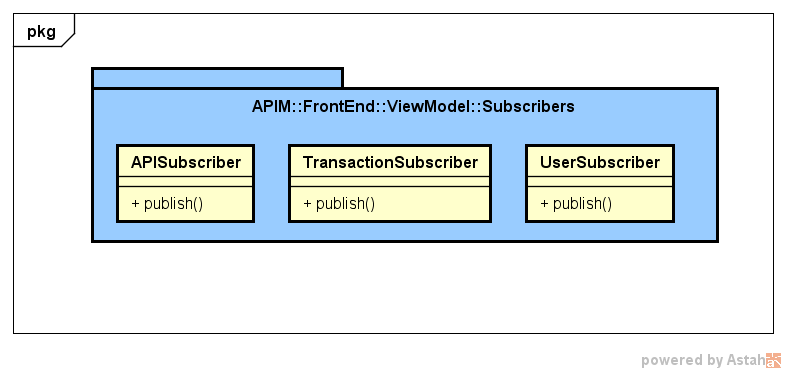
\includegraphics
	[width=0.7\linewidth]
	{UML/DiagrammiPackage/Subscribers.png}
	\caption{Package APIM::FrontEnd::ViewModel::Subscribers}
\end{figure}

\subparagraph{APISubscriber}
\begin{itemize}
	\item \textbf{Funzione del componente}: la classe esegue il subscribing delle API.
	\item \textbf{Relazioni d’uso di altri componenti}: è in relazione con l'APIController.
	\item \textbf{Attività svolte e dati trattati}: esegue il subscribing di quelle collezioni di cui è stato precedentemente fatto il publishing.
\end{itemize}

\subparagraph{TransactionSubscriber}
\begin{itemize}
	\item \textbf{Funzione del componente}: la classe esegue il subscribing delle transazioni.
	\item \textbf{Relazioni d’uso di altri componenti}: è in relazione con il TransactionController.
	\item \textbf{Attività svolte e dati trattati}: esegue il subscribing di quelle collezioni di cui è stato precedentemente fatto il publishing.
\end{itemize}

\subparagraph{UserSubscriber}
\begin{itemize}
	\item \textbf{Funzione del componente}: la classe esegue il subscribing degli utenti.
	\item \textbf{Relazioni d’uso di altri componenti}: è in relazione con lo UserController.
	\item \textbf{Attività svolte e dati trattati}: esegue il subscribing di quelle collezioni di cui è stato precedentemente fatto il publishing.
\end{itemize}

\paragraph{Methods}

\begin{figure}[H]
	\centering
	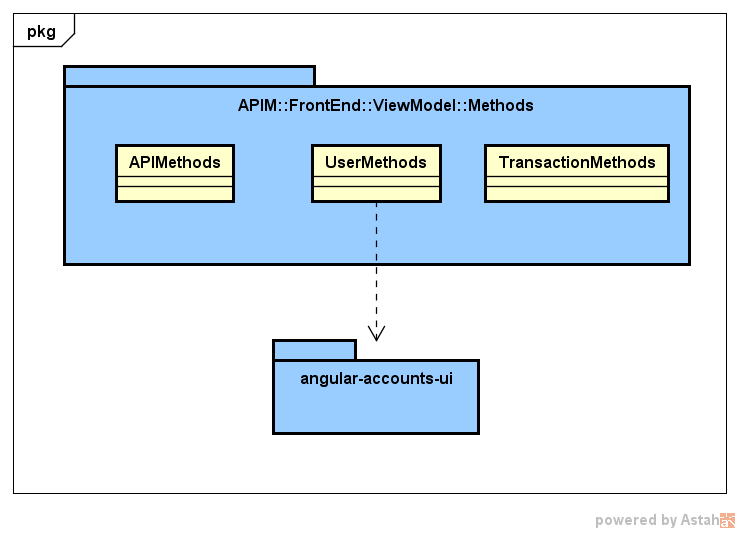
\includegraphics
	[width=0.7\linewidth]
	{UML/DiagrammiPackage/Methods.png}
	\caption{Package APIM::FrontEnd::ViewModel::Methods}
\end{figure}

\subparagraph{APIMethods}
\begin{itemize}
	\item \textbf{Funzione del componente}: la classe viene utilizzata dal Frontend per richiedere una modifica delle API.
	\item \textbf{Relazioni d’uso di altri componenti}: è in relazione con NewAPIController e EditAPIController.
	\item \textbf{Attività svolte e dati trattati}: fornisce all'utente le funzioni di inserimento, modifica e cancellazione delle API.
\end{itemize}

\subparagraph{TransactionMethods}
\begin{itemize}
	\item \textbf{Funzione del componente}: la classe viene utilizzata dal Frontend per richiedere una modifica delle transazioni.
	\item \textbf{Relazioni d’uso di altri componenti}: è in relazione con NewTransactionController e EditTransactionController.
	\item \textbf{Attività svolte e dati trattati}: fornisce all'utente le funzioni di inserimento, modifica e cancellazione delle transazioni.
\end{itemize}

\subparagraph{UserMethods}
\begin{itemize}
	\item \textbf{Funzione del componente}: la classe viene utilizzata dal Frontend per richiedere una modifica degli utenti.
	\item \textbf{Relazioni d’uso di altri componenti}: è in relazione con il package esterno angular-accounts-ui.
	\item \textbf{Attività svolte e dati trattati}: fornisce all'utente le funzioni di inserimento, modifica e cancellazione degli utenti.
\end{itemize}


\paragraph{Routers}

\begin{figure}[H]
	\centering
	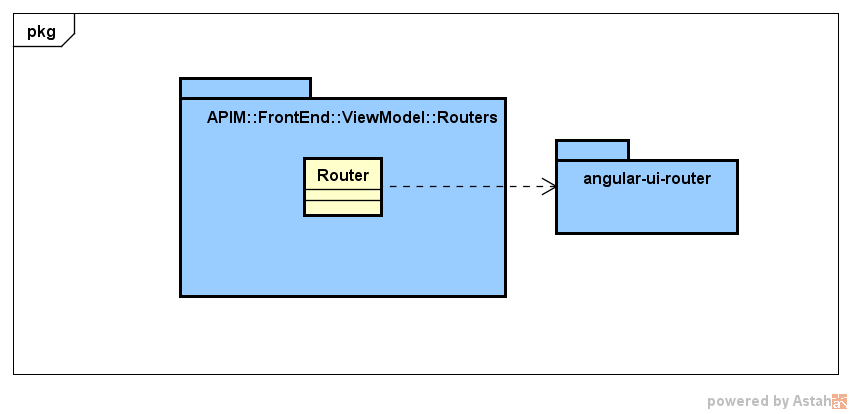
\includegraphics
	[width=0.7\linewidth]
	{UML/DiagrammiPackage/Routers.png}
	\caption{Package APIM::FrontEnd::ViewModel::Routers}
\end{figure}

\subparagraph{Router}
\begin{itemize}
	\item \textbf{Funzione del componente}: la classe permette il routing dinamico delle pagine.
	\item \textbf{Relazioni d’uso di altri componenti}: è in relazione con il package esterno angular-ui-router e con tutte le pages e i templates.
	\item \textbf{Attività svolte e dati trattati}: esegue la traduzione degli URL in modo dinamico, permettendo la visualizzazione in modalità one-page, senza bisogno di ricaricare l'intera pagina.
\end{itemize}
\newpage
\subsection{Back-end}

Il lato back-end risulta così strutturato:

\begin{figure}[H]
	\centering
	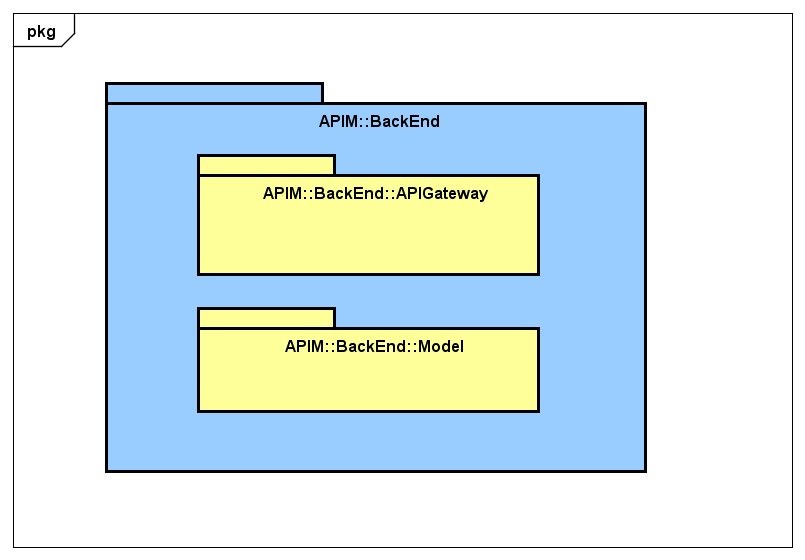
\includegraphics
	[width=0.7\linewidth]
	{UML/DiagrammiPackage/BackEnd.png}
	\caption{Package APIM::BackEnd}
\end{figure}

Nella parte back-end sono dunque presenti i package APIGateway e Model strutturati secondo un'architettura a microservizi.


\begin{figure}[H]
	\centering
	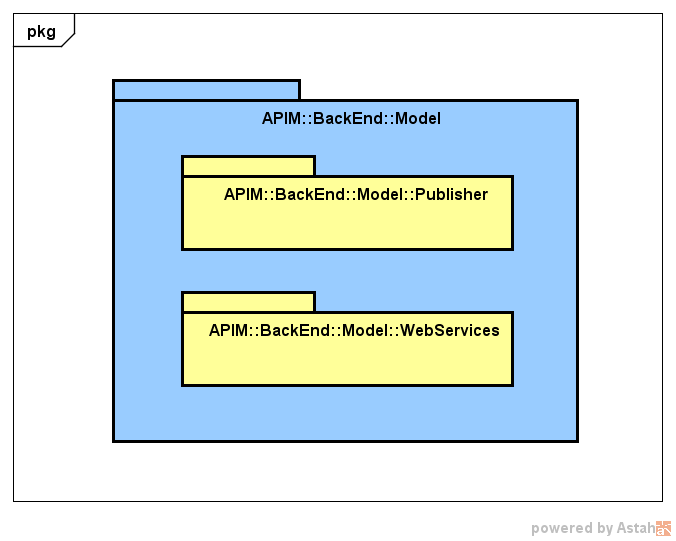
\includegraphics
	[width=0.7\linewidth]
	{UML/DiagrammiPackage/Model.png}
	\caption{Package APIM::BackEnd::Model}
\end{figure}

Il package \textit{Model} contiene i packages utilizzati per rappresentare i dati e l'implementazione della logica di business e di validazione.
\begin{itemize}
	\item \textbf{Publisher}: contiene le classi per la pubblicazione dei dati;
	\item \textbf{WebServices}: contiene le classi per la comunicazione col database.
\end{itemize}


\subsubsection{Publisher}
\begin{figure}[H]
	\centering
	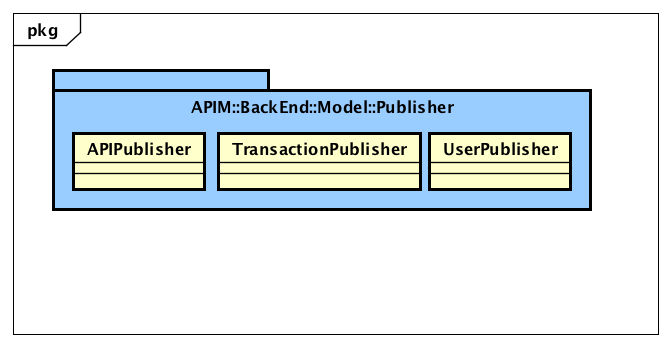
\includegraphics
	[width=0.7\linewidth]
	{UML/DiagrammiPackage/Publisher.png}
	\caption{Package APIM::BackEnd::Model::Publisher}
\end{figure}

Il package \textit{Publisher} contiene le classi necessarie ad esporre il modello dati al front-end.

\paragraph{APIPublisher}
\begin{itemize}
	\item \textbf{Funzione del componente}: esegue la pubblicazione delle API;
	\item \textbf{Attività svolte e dati trattati}: permette l'accesso alla collezione di API.
\end{itemize}

\paragraph{TransactionPublisher}
\begin{itemize}
	\item \textbf{Funzione del componente}: esegue la pubblicazione delle transazioni;
	\item \textbf{Attività svolte e dati trattati}: permette l'accesso alla collezione di transazioni.
\end{itemize}

\paragraph{UserPublisher}
\begin{itemize}
	\item \textbf{Funzione del componente}: esegue la pubblicazione degli utenti;
	\item \textbf{Attività svolte e dati trattati}: permette l'accesso alla collezione di utenti.
\end{itemize}


\subsubsection{WebServices}

\begin{figure}[H]
	\centering
	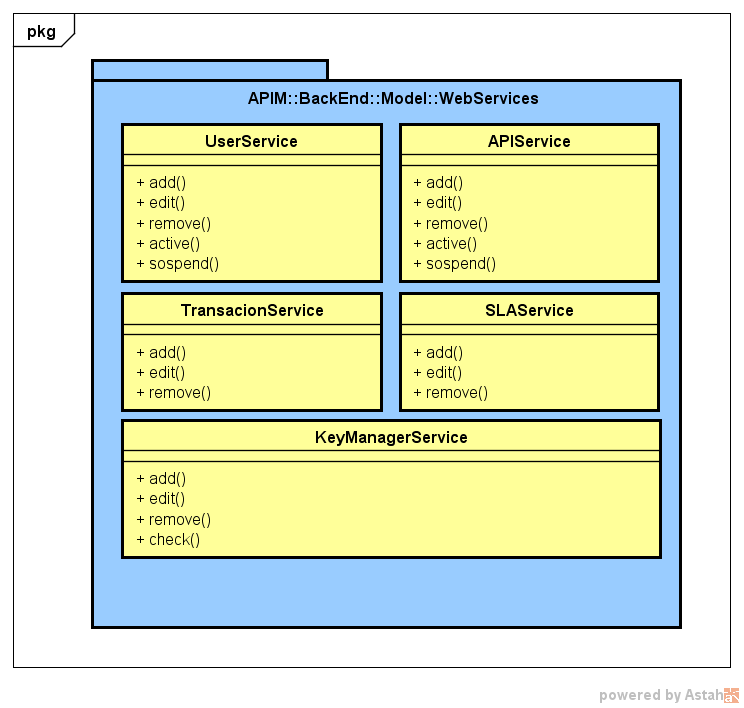
\includegraphics
	[width=0.7\linewidth]
	{UML/DiagrammiPackage/WebServices.png}
	\caption{Package APIM::BackEnd::Model::WebServices}
\end{figure}

Il package \textit{WebServices} contiene i microservizi utilizzati per mettere in comunicazione il database con il \textit{Model}.

\paragraph{UserService}
\begin{itemize}
	\item \textbf{Funzione del componente}: esegue le funzioni di inserimento, modifica e rimozione di utenti;
	\item \textbf{Relazioni d'uso di altri componenti}: si interfaccia con il \textit{ViewModel} e il database per fornire le funzioni di inserimento, modifica e rimozione di utenti.
\end{itemize}

\paragraph{APIService}
\begin{itemize}
	\item \textbf{Funzione del componente}: esegue le funzioni di inserimento, modifica e rimozione di API;
	\item \textbf{Relazioni d'uso di altri componenti}: si interfaccia con il \textit{ViewModel} e il database per fornire le funzioni di inserimento, modifica e rimozione di API.
\end{itemize}

\paragraph{TransactionService}
\begin{itemize}
	\item \textbf{Funzione del componente}: esegue le funzioni di inserimento, modifica e rimozione di transazioni;
	\item \textbf{Relazioni d'uso di altri componenti}: si interfaccia con il \textit{ViewModel} e il database per fornire le funzioni di inserimento, modifica e rimozione di transazioni.
\end{itemize}


\paragraph{SLAService}
\begin{itemize}
	\item \textbf{Funzione del componente}: esegue le funzioni di inserimento, modifica e rimozione di log di SLA;
	\item \textbf{Relazioni d'uso di altri componenti}: si interfaccia con il \textit{ViewModel} e il database per fornire le funzioni di inserimento, modifica e rimozione di log di SLA.
\end{itemize}

\paragraph{KeyManagerService}
\begin{itemize}
	\item \textbf{Funzione del componente}: esegue le funzioni di inserimento, modifica e rimozione di API key;
	\item \textbf{Relazioni d'uso di altri componenti}: si interfaccia con il \textit{ViewModel} e il database per fornire le funzioni di inserimento, modifica e rimozione di API key.
\end{itemize}


\newpage
\section{API Gateway}





%\newpage
\section{Diagrammi di attività}
\subsection{Introduzione}
I diagrammi di attività sono diagrammi che descrivono un processo. Il diagramma di attività modella un processo. Organizza più entità in un insieme di azioni secondo un determinato flusso.
Il gruppo ha deciso di prendere in esame tre possibili situazioni rilevanti all'interno dell'API Market.

\subsection{Diagramma di attività relativa alla ricerca di una API}
\begin{figure} [H]
	\centering
	\includegraphics[width=1.0\linewidth]{"IMG/ricerca API"}
	\caption{Diagramma di attività che descrive la ricerca di una API}
\end{figure}
\begin{itemize}
	\item \textbf{Precondizioni}: l'utente si trova all'interno dell'API Market e decide di effettuare una ricerca di una API in base ad alcuni parametri;
	\item \textbf{Postcondizioni}: l'Utente ha individuato l'API adatta al suo scopo e potrà acquistarla(vedi diagramma "Acquisto API");
	\item \textbf{Descrizione}: l'utente riempie un box di ricerca con i termini desiderati e in una nuova pagina visualizza le API corrispondenti ai parametri inseriti. Attualmente all'utente si presentano due possibili scelte: Effettuare una nuova ricerca con parametri diversi se i risultati della ricerca non soddisfano le sue aspettative oppure visualizzare la pagina dedicata ad una API. All'interno di una API si presentano tre possibili scenari: se l'utente è soddisfatto dell'API può decidere di proseguire l'acquisto, situazione descritta nel diagramma "Acquisto API" oppure ha due alternative: ritornare ai risultati della ricerca precedente o effettuare una nuova ricerca.
\end{itemize}

\newpage
\subsection{Diagramma di attività relativa all'acquisto di una API}
\begin{figure}[h]
	\centering
	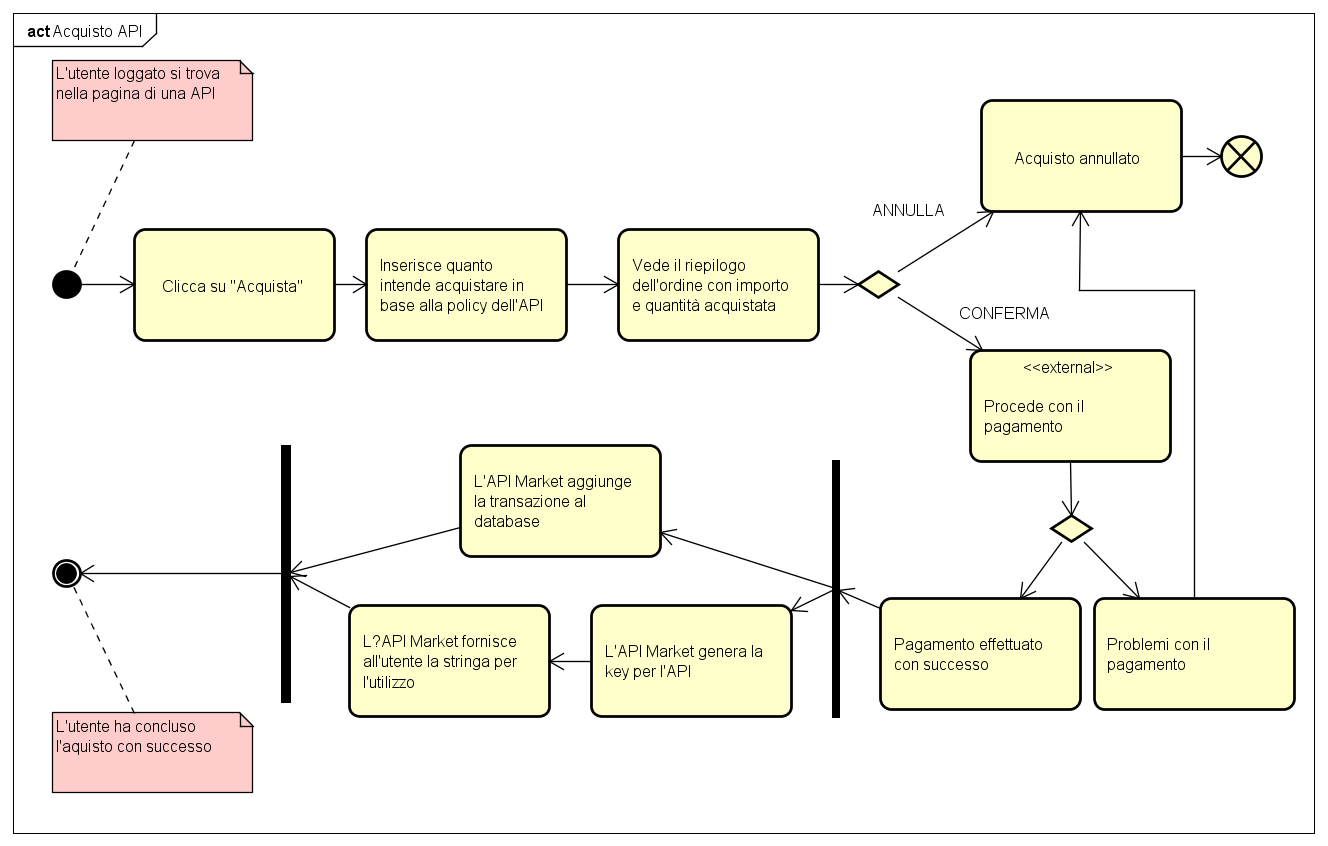
\includegraphics[width=1.0\linewidth]{IMG/Acquisto_API}
	\caption{}
	\label{fig:acquistoapi}
\end{figure}

\begin{itemize}
	\item \textbf{Precondizioni}: L'utente ha scelto un'API dal Market e vuole acquistarla;
	\item \textbf{Postcondizioni}: L'utente ha acquistato un'API e può utilizzarla;
	\item \textbf{Descrizione}: Inizialmente l'utente si trova nella pagina dell'API che desidera acquistare. Una volta cliccato su acquista inserisce la quantità che vuole acquistare in base alla policy prevista per quell'API. Successivamente vedrà un riepilogo dell'acquisto, contenente importo in euro e la quantità espressa in base alla policy, ovvero il numero di chiamate, la quantità di traffico espressa in kB oppure il tempo espresso in minuti. L'utente può decidere se confermare il pagamento con un checkout esterno sul sito di Paypal oppure annullare l'ordine. Il pagamento avviene su un sito esterno ed è possibile che la transazione non vada a buon fine quindi è previsto il caso in cui l'utente abbia problemi con il pagamento e quindi l'acquisto venga annullato. Una volta che l'acquisto è confermato, l'API Market aggiungere la transazione al database, genera la chiave e fornisce all'utente l'indirizzo e la stringa da utilizzare per chiamare l'API, terminando l'acquisto con successo. 
\end{itemize}

\newpage
\subsection{Diagramma di attività relativa all'inserimento di una API}
\begin{figure}[h]
	\centering
	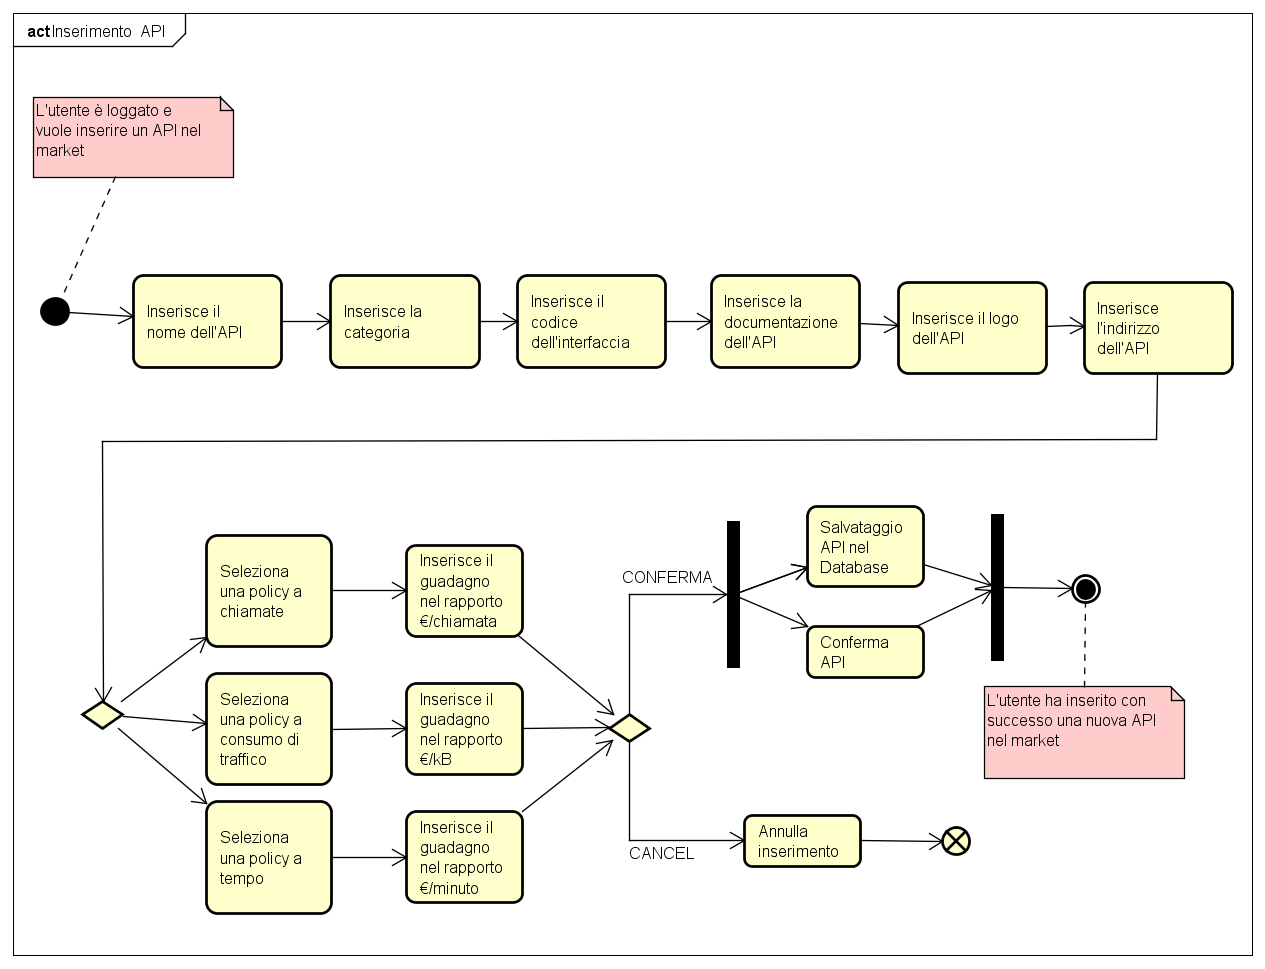
\includegraphics[width=1.0\linewidth]{IMG/Inserimento_API}
	\caption{}
	\label{fig:inserimentoapi}
\end{figure}


\begin{itemize}
	\item \textbf{Precondizioni}: L'utente ha sviluppato un'api e si trova nel suo profilo con l'intenzione di pubblicarla sul Market;
	\item \textbf{Postcondizioni}: L'utente ha aggiunto un'API al Market;
	\item \textbf{Descrizione}: L'utente si trova nel suo profilo e tramite il pulsante aggiungi API, carica una sua API sul Market. L'utente visualizza in una nuova pagina una serie di campi in cui inserire i dati richiesti per la sua API. Questi dati sono i seguenti
	\begin{itemize}
		\item Il nome dell'API;
		\item la Categoria di appartenenza dell'API;
		\item Il codice dell'interfaccia dell'API;
		\item La documentazione dell'API;
		\item Il logo dell'API;
		\item L'indirizzo dell'API;
		\item Sceglie la policy e il guadagno della sua API, ovvero:
		\begin{itemize}
			\item \textbf{Policy a chiamate}: definisce il guadagno espresso in euro per ogni chiamata da parte di un acquirente della sua API;
			\item \textbf{Policy a traffico}: definisce il guadagno espresso in euro per ogni kB trasmesso all'acquirente sua API;
			\item \textbf{Policy a tempo}: definisce il guadagno espresso in euro per ogni minuto di utilizzo da parte di un acquirente della sua API.
		\end{itemize}		
	\end{itemize}
	Successivamente può decidere se annullare il caricamento oppure confermarlo. Una volta inviata la conferma, l'API Market restituisce una conferma e salva l'API nel Database, rendendola disponibile all'acquisto da parte dei fruitori dell'API Market.
\end{itemize}

\newpage
\section{Diagrammi di sequenza}
\subsection{Introduzione}
Un Diagramma di sequenza) è un diagramma previsto dall'UML utilizzato per descrivere uno scenario.
Uno scenario è una determinata sequenza di azioni in cui tutte le scelte sono state già effettuate; in pratica nel diagramma non compaiono scelte, né flussi alternativi.
Il gruppo ha deciso di prendere in esame la situazione di chiamata all'API Gateway suddividendo la sequenza in due parti.

\subsection{Diagramma di sequenza relativa alla chiamata di una API}
\subsubsection{Diagramma di sequenza di gestione della chiamata}
\begin{figure}[h]
	\centering
	\includegraphics[width=1.0\linewidth]{"IMG/Sequence Diagram0"}
	\caption{Diagramma di sequenza di gestione della chiamata}
\end{figure}

\begin{itemize}
	\item \textbf{Precondizioni}: Il client ha effettuato una chiamata ad una API;
	\item \textbf{Postcondizioni}: La richiesta arriva all'API Gateway Manager che la processa;
	\item \textbf{Descrizione}: il client effettua una chiamata creando un oggetto API Call. L'oggetto API Call viene aggiunto alla coda QueueAPICall in attesa di essere prelevato dall'API Gateway Manager per la sua esecuzione. Quando la chiamata verrà processata i suoi dati verranno salvati nel Buffer.
\end{itemize}

\newpage
\subsubsection{Diagramma di sequenza dell'API Gateway Manager}
\begin{figure}[h]
	\centering
	\includegraphics[width=1.0\linewidth]{"IMG/Sequence Diagram1"}
	\caption{Diagramma di sequenza dell'API Gateway Manager}
\end{figure}


\begin{itemize}
	\item \textbf{Precondizioni}: La richiesta arriva all'API Gateway Manager che la processa;
	\item \textbf{Postcondizioni}: Il client riceve la risposta alla sua chiamata e i dati relativi alla SLA, se abilitata, sono stati salvati nel Database;
	\item \textbf{Descrizione}: L'API Gateway Manager invoca i metodi del Verifier per eseguire i controlli necessari per verificare l'autenticità della chiamata. All'interno del Verifier viene deciso in modo casuale se effettuare il log della SLA.
	Conclusi questi controlli preliminari con successo, il Manager invoca i metodi di RequestForwarder che si occupano di recuperare l'indirizzo dell'API invocata ed salvarlo nel Service Registry, effettua un salvataggio relativo alla SLA e conclude la sua esecuzione con la chiamata all'API target. Il Manager invoca i metodi del ResponseForwarder, il quale si occupa di effettuare il salvataggio relativo alla SLA, diminuire il campo Residue nel Database e inviare la risposta al Client chiamante. Infine il Manager si occupa di salvare il record della SLA nel Database.  
\end{itemize}

\newpage
\renewcommand*{\arraystretch}{1.6}

\section{Tracciamento}
\subsection{Mappatura componenti-requisiti}



		\begin{longtable}{ p{12cm} | p{4cm} }
			\hline
			\textbf{Nome Componente} & \textbf{Codice Requisito} \\
			\hline
			APIM::FrontEnd::View::Pages::ProfilePage& RFO10.1 \\
			& RFO10.1.1 \\
			& RFO10.1.2 \\
			& RFO10.1.3 \\
			& RFO10.1.4 \\
			& RFO10.1.5 \\
			& RFO10.1.6 \\
			& RFO10.1.2.1 \\
			& RFO10.1.2.2 \\
			& RFO10.1.2.3 \\
			& RFO10.1.2.4 \\
			& RFO10.1.2.5 \\
			& RFO10.1.2.6 \\
			& RFO10.1.2.7 \\
			& RFO10.1.2.8 \\
			& RFO10.1.2.8 \\
			& RFO10.1.2.8 \\
			&RFO10.2.1 \\
			&RFO10.2.2 \\
			&RFO10.2.2.1 \\
			&RFO10.2.2.2 \\
			&RFO10.3 \\
			&RFO10.3.1 \\
			&RFO10.3.1.1 \\
			&RFO10.3.1.2 \\
			&RFO10.3.2 \\
			\hline
			APIM::FrontEnd::View::Pages::RegistrationPage& RFO10.1 \\
			&RFO1 \\
			&RFO1.1 \\
			&RFO1.2 \\
			&RFO1.3 \\
			&RFO1.4 \\
			&RFO1.5 \\
			&RFO1.6 \\
			&RFO1.7 \\
			&RFO1.8 \\
			&RFO1.9 \\
			&RFO1.10 \\
			\hline
			APIM::FrontEnd::View::Pages::LoginPage& RFO10.1 \\
			&RFO2 \\
			&RFO2.1 \\
			&RFO2.1.1\\
			&RFO2.1.2\\
			&RFO2.1.3\\
			&RFO2.1.4\\
			&RFF2.2\\
			&RFF2.2.2\\
			&RFF2.3\\
			&RFF2.3.2\\
			&RFF2.4\\
			&RFF2.4.2\\
			&RFF2.5\\
			&RFF2.5.2\\
			\hline
			APIM::FrontEnd::View::Pages::Index& RFO10 \\
			&RFO1 \\
			&RFO1.1 \\
			&RFO1.2 \\
			&RFO1.3 \\
			&RFO1.4 \\
			&RFO1.5 \\
			&RFO1.6 \\
			&RFO1.7 \\
			&RFO1.8 \\
			&RFO1.9 \\
			&RFO1.10 \\
			&RFO2 \\
			&RFO2.1 \\
			&RFO2.1.1\\
			&RFO2.1.2\\
			&RFO2.1.3\\
			&RFO2.1.4\\
			&RFF2.2\\
			&RFF2.2.2\\
			&RFF2.3\\
			&RFF2.3.2\\
			&RFF2.4\\
			&RFF2.4.2\\
			&RFF2.5\\
			&RFF2.5.2\\
			
			\hline
			APIM::FrontEnd::View::Pages::AdministrationPage& RFO10 \\
			&RFO12\\
			&RFO12.1\\
			&RFO12.1.1\\
			&RFO12.1.1.1\\
			&RFO12.1.1.1.1\\
			&RFO12.1.1.1.2\\
			&RFD12.1.1.1.3\\
			&RFD12.1.1.1.4\\
			&RFO12.1.1.1.5\\
			&RFO12.1.1.1.5.1\\
			&RFF12.1.1.1.5.2\\
			&RFD12.1.1.1.6\\
			&RFO12.1.1.2\\
			&RFO12.1.1.2.1\\
			&RFO12.1.1.2.2\\
			&RFD12.1.1.3\\
			&RFD12.1.1.3.1\\
			&RFD12.1.1.3.2\\
			&RFO12.1.1.3.3\\
			&RFO12.2\\
			&RFO12.2.1\\
			&RFO12.2.1.1\\
			&RFO12.2.1.1.1\\
			&RFO12.2.1.1.2\\
			&RFO12.2.1.2\\
			&RFO12.2.1.2.1\\
			&RFO12.2.1.2.2\\
			&RFO12.2.1.3\\
			&RFO12.2.1.4\\
			&RFO12.2.1.5\\
			&RFO12.2.1.5.1\\
			&RFO12.2.1.5.2\\
			&RFO12.2.1.2.2\\
			\hline
			APIM::FrontEnd::View::Pages::APIPage& RFO10 \\
			&RFO4.3.1\\
			&RFO4.3.2\\
			&RFO4.3.3\\
			&RFD4.3.4\\
			&RFO4.3.5\\
			&RFO5\\
			&RFO5.1\\
			&RFO5.2\\
			&RFO5.3\\
			&RFO5.4\\
			&RFO5.5\\
			&RFO5.5.1\\
			&RFO5.5.2\\
			&RFO5.6\\
			&RFO5.6.1\\
			&RFD5.6.2\\
			&RFO5.7\\
			&RFD5.7.1\\
			&RFO5.7.2\\
			&RFO5.8\\
			&RFO5.9\\
			&RFO5.10\\
			&RFD5.11\\
			&RFO5.12\\
			&RFO5.13\\
			&RFO6\\
			&RFO6.1\\
			&RFO6.2\\
			&RFO6.2.1\\
			&RFO6.2.2\\
			&RFO6.2.3\\
			&RFO6.2.4\\
			&RFO6.2.5\\
			&RFO6.2.6\\
			&RFO6.2.7\\
			&RFO7\\
			&RFO7.1\\
			&RFO7.1.1\\
			&RFO7.1.2\\
			&RFO7.1.3\\
			&RFO7.2\\
			&RFO7.3\\
			&RFO7.4\\
			&RFO7.5\\
			&RFD7.5.1\\
			&RFO7.5.2\\
			&RFO7.5.3\\
			&RFO7.6\\
			&RFO8\\
			&RFO8.1\\
			&RFO8.2\\
			&RFO8.2.1\\
			&RFO8.2.2\\
			&RFO8.2.3\\
			&RFO8.2.4\\
			&RFO8.2.4.1\\
			&RFO8.2.4.2\\
			&RFD8.2.4.3\\
			&RFD8.2.4.4\\
			&RFD8.2.4.5\\
			&RFD8.2.4.6\\
			&RFD8.2.4.7\\
			&RFD8.2.4.8\\
			&RFD8.2.4.9\\
			&RFD8.2.4.10\\
			&RFD8.2.4.11\\
			&RFD8.2.5\\
			&RFD8.2.6\\
			&RFD8.2.7\\
			&RFO8.2.8\\
			&RFO8.2.9\\
			&RFO8.2.9.1\\
			&RFO8.2.9.2\\
			&RFO9\\
			&RFO9.1\\
			&RFO9.2\\
			&RFD9.3\\
			&RFO9.4\\
			&RFO9.5\\
			&RFD9.6\\
			&RFD9.7\\
			&RFO9.8\\
			&RFO9.8.1\\
			&RFO9.8.2\\
			&RFO9.8.3\\
			&RFO9.9\\
			&RFD9.10\\
			&RFD9.11\\
			&RFO9.12\\
			&RFD9.13\\
			\hline
		    APIM::FrontEnd::View::Pages::SearchPage& RFO10 \\
		    &RFO4\\
		    &RFO4.1\\
		    &RFO4.2\\
		    &RFO4.3\\
		    &RFO4.3.1\\
		    &RFO4.3.2\\
		    &RFO4.3.3\\
		    &RFD4.3.4\\
		    &RFO4.3.5\\
		    \hline
		    APIM::FrontEnd::View::Pages::CategoryListPage& RFO10 \\
		    &RFO5.4\\
		    
		    \hline
		    APIM::FrontEnd::View::Templates::MainMenu& RFO10 \\
		    \hline
		    APIM::FrontEnd::View::Templates::SearchForm& RFO10 \\
		    \hline
		    APIM::FrontEnd::View::Templates::UserList& RFO10 \\		 
		    \hline   
		    APIM::FrontEnd::View::Templates::User& RFO10 \\	
		    \hline	    
		    APIM::FrontEnd::View::Templates::UserMenu& RFO10 \\	
		    \hline	    
		    APIM::FrontEnd::View::Templates::SearchResult& RFO10 \\	
		    \hline	    
		    APIM::FrontEnd::View::Templates::MyAPIList& RFO10 \\
		    \hline		    
		    APIM::FrontEnd::View::Templates::LoginForm& RFO10 \\	
		    \hline	    
		    APIM::FrontEnd::View::Templates::APIList& RFO10 \\
		    \hline	
		    APIM::FrontEnd::View::Templates::API& RFO10 \\
		    \hline	
		    APIM::FrontEnd::View::Templates::RegistrationForm& RFO10 \\
		    \hline	
		    APIM::FrontEnd::View::Templates::CategoryList& RFO10 \\
		    \hline	
		    APIM::FrontEnd::View::Templates::Category& RFO10 \\
		    \hline	APIM::FrontEnd::View::Templates::PasswordRecoveryForm& RFO10 \\	
		    APIM::FrontEnd::View::Templates::APIRegistrationForm& RFO10 \\	
		    \hline
		    APIM::FrontEnd::View::Templates::TransactionList& RFO10 \\
		    \hline	
		    APIM::FrontEnd::View::Templates::Transaction& RFO10 \\
		    \hline	
		    APIM::FrontEnd::View::Templates::APIEditForm& RFO10 \\	
		    \hline
		    APIM::FrontEnd::View::Templates::EditProfileForm& RFO10 \\	
		    \hline
		    APIM::FrontEnd::View::Templates::CheckoutForm& RFO10 \\
		    \hline
		    APIM::FrontEnd::ViewModel::Controllers::MenuController& FO10 \\
		    \hline	
		    APIM::FrontEnd::ViewModel::Controllers::CategoryController& FO10 \\
		    \hline	
		    APIM::FrontEnd::ViewModel::Controllers::CheckoutController& FO10 \\
		    \hline	
		    APIM::FrontEnd::ViewModel::Controllers::UserListController& FO10 \\
		    \hline	
		    APIM::FrontEnd::ViewModel::Controllers::ManageProfileController& FO10 \\
		    \hline	
		    APIM::FrontEnd::ViewModel::Controllers::CategoryListController& FO10 \\
		    \hline	
		    APIM::FrontEnd::ViewModel::Controllers::TransactionController& FO10 \\	
		    \hline
		    APIM::FrontEnd::ViewModel::Controllers::NewPolicyController& FO10 \\
		    \hline	
		    APIM::FrontEnd::ViewModel::Controllers::SearchController& FO10 \\
		    \hline	
		    APIM::FrontEnd::ViewModel::Controllers::NewAPIController& FO10 \\
		    \hline
		    APIM::FrontEnd::ViewModel::Controllers::TransactionListController& FO10 \\
		    \hline
		    APIM::FrontEnd::ViewModel::Controllers::EditPolicyController& FO10 \\
		    \hline
		    APIM::FrontEnd::ViewModel::Controllers::APIController& FO10 \\
		    \hline
		    APIM::FrontEnd::ViewModel::Controllers::EditAPIController& FO10 \\
		    \hline
		    APIM::FrontEnd::ViewModel::Controllers::UserController& FO10 \\
		    \hline
		    APIM::FrontEnd::ViewModel::Controllers::PolicyListController& FO10 \\
		    \hline
		    APIM::FrontEnd::ViewModel::Controllers::APIListController& FO10 \\
		    \hline
		    APIM::FrontEnd::ViewModel::Subscribers::APISubscriber& FO10 \\
		    \hline
		    APIM::FrontEnd::ViewModel::Subscribers::TransactionSubscriber& FO10 \\
		    \hline
		    APIM::FrontEnd::ViewModel::Subscribers::UserSubscriber& FO10 \\
		    \hline
		    APIM::FrontEnd::ViewModel::Methods::APIMethods& FO10 \\
		    \hline
		    APIM::FrontEnd::ViewModel::Subscribers::UserMethods& FO10 \\
		    \hline
		    APIM::FrontEnd::ViewModel::Subscribers::TransactionMethods& FO10 \\
		    \hline
		    APIM::FrontEnd::ViewModel::Routers::Router& FO10 \\
		    \hline
		   
		
		\end{longtable}




\end{document}